
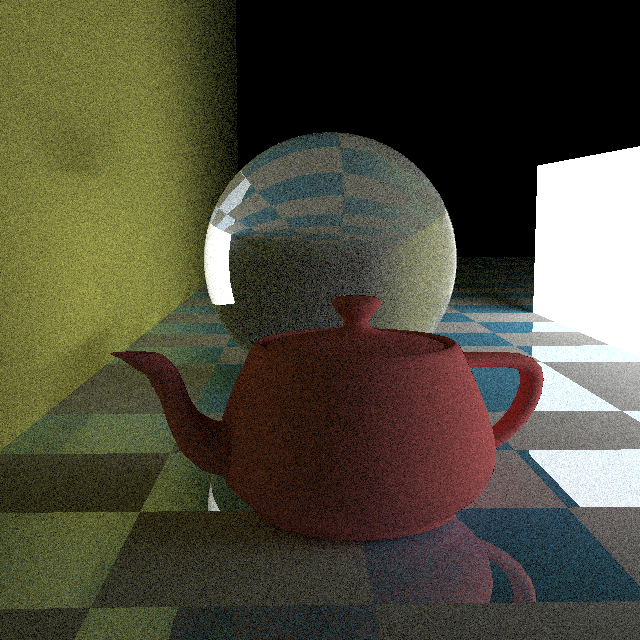
\includegraphics[width=0.5\textwidth]{img/teapot-in-front-of-sphere.png}

\section{About the team}
The first two assignments were done with Nick Begg.
Not this assignment, as we both wanted to learn different things.
We forked off right after the second assignment to work on our own raytracer.

\section{New Features}
For the final assignment I made a realtime pathtracer with:
\begin{enumerate}
    \item Awesome materials:
        \begin{enumerate}
            \item Area lights as material, every object with a non-zero emissive component in its \verb:.mtl: file is an area light.
                  When the scene is loaded, all emissive triangles have their index recorded in an array.
            \item reflective materials.
            \item transparent, refractive materials.
            \item diffuse materials.
            \item Fresnell's angle dependent transparency
            \item Materials can have any amount of reflectiveness, transparancy and difuseness at the same time.
                  The ray computes the probabilities to reflect like a mirror, refract, or reflect in a diffuse way.
            \item You can combine two arbitrary materials together into a checkerboard pattern!
        \end{enumerate}
    \item Next Event Estimation. 
        The path tracer returns the sum of two functions, \verb:directIllumination: and \verb:indirectIllumination:. 
        \verb:directIllumination: launches a ray toward a random point on a random light emiting triangle.
        \verb:indirectIllumination: is the pathtracer propper, it bounces off (or into) the material and recursively calls the pathtracer.
    \item Importance Sampling.
        The diffuse bounce is implemented with a random cosine-weighted distribution.
    \item Intuitive controls: 
        \begin{enumerate}
            \item WASD for forward, backward and strafing.
            \item Space for going up.
            \item Shift for going down.
        \end{enumerate}
    \item The ability to load gzipped \verb:.obj: files.
    \item A XorShift32 random number generator (before it was cool, I implemented it before the slides on random number generators).
    \item Optional Color Correction. It defaults to on, press L to toggle it.
    \item A new performance view that shows the pathtrace performance instead of the whitted-style performance (press 8).
    \item Toggelable mouse release, press Q to free your mouse.
    \item A resizable window! Now that you can toggle mouse capturing, you can resize the window to your hearts content.
\end{enumerate}




\section{Old Features from the Whitted-style raytracer}
Features that were already in the raytracer from assignment 2, for completeness' sake.

\subsection{BVH building}
3 BVH construction methods are available in the project -
    \begin{enumerate}
        \item Stupid: Builds a 'no-op' BVH; It will have a single root node containing all primitives. This will thus force a linear traversal of all triangles, giving almost the performance of the original assignment 1 ray tracer (although as it contains a bounding box, rays that miss the geometry entirely will be accelerated).
        \item Standard BVH: A standard BVH, constructed using the surface-area heuristic (SAH) against the longest axis of the set of primitives.
        \item SBVH: A split BVH which implements both OBJECT and SPATIAL splits against all 3 axis, "reference unsplitting" and spatial split attempt reduction.
    \end{enumerate}

\subsection{BVH traversal}
Both an ordered and unordered traversal mode is available (ordered is the default).

\subsection{Whitted-style raytracer materials}
    \begin{enumerate}
    \item diffuse lighting with hard shadows
    \item reflections
    \item transparency with refraction indices
    \item specular highlights
    \item diffuse, reflective and specular values are defined by a 3-value color to match the \verb|.mtl| file format
    \item they can also be combined in arbitrary ways (i.e.\ a material can have a diffuse, reflective, transparent and specular components)
    \item triangle meshes support smoothing using barycentric interpolation of the vertex normals
    \end{enumerate}

\subsection{Run time scene loader}
    \begin{enumerate}
    \item Json scene loader
        \begin{enumerate}
        \item Triangle meshes --- loaded from file, and transformed into the world (translate, rotate, scale)
        \item Point and Spot lights
        \item camera
        \end{enumerate}
    \item \verb|.obj| file loader (using tinyojb)
    \item \verb|.mtl| material file loader (using tinyobj)
    \end{enumerate}

\subsection{Camera}
    \begin{enumerate}
    \item zoom (mousewheel)
    \item pitch, yaw and translate
    \end{enumerate}

\subsection{Whitted-style raytracer lights}
    \begin{enumerate}
    \item multi-color lighting
    \item point lights
    \item spot lights with linear falloff
    \end{enumerate}

\subsection{Other}
    \begin{enumerate}
    \item multi-platform with CMake (linux, mac and windows)
    \item multi-threaded with OpenMP (got around 5x speedup on linux, which is what is expected for 4 cores with Hyperthreading)
    \end{enumerate}

\section{Building}

\subsection{Building on Windows}
A visual studio solution is provided (ray.sln). This project was tested and built under Visual Studio 2015 Community. 

It should be a matter of simply loading the solution file into Visual Studio, and building. A release build is recommended as it is significantly faster.

NOTE: only 32bit (ie x86) builds have been tested. Make sure this is selected when building.

\subsection{Building with Cmake}
The source can be built using the standard CMake environment. This will work on Windows, macOS and Linux. 

For example, on unix systems this command will perform a release build -

\verb|cmake -DCMAKE_BUILD_TYPE=Release . ;| \\
\verb|make|

A similar command should work with Visual Studio, although the \verb|CMAKE_BUILD_TYPE| is not required - this is set in the Visual Studio gui.

Boost is required for the test tree, but not the main system.

\section{Running}

On Windows, SDL2.dll must be available somewhere on the path or in the same dir as the binary. 

There is a collection of test scenes, objects and materials in the data directory. To avoid fighting with relative paths, it works best to cd to this directory before running the system. For example, on windows, assuming the binary is in the Release directory under the root source tree - 

\verb|cd <source_root>| \\
\verb|..\Release\ray.exe teapot-plane.scene|

\section{Controls}
    \begin{tabular}{ll}
    \hline
    WASD & move forward, backward, and strafe \\
    Shift & move down \\
    Space & move up \\
    mouse & rotate camera (yaw/pitch) \\
    mouse wheel & zoom in/out (changes FOV) \\
    \hline
    Esc & quit \\
    P   & write screenshot image \\
    R   & reset camera view to default (set from scene file) \\
    C   & print the current camera parameters \\
    M   & Toggle barycentric smoothing \\
    B   & change BVH construction method \\
    T   & change BVH traversal method (ordered/unordered) \\
    Q   & release mouse \\
    \hline
    9   & view path-traced image (default) \\
    8   & visualise per-pixel render time for the path tracer. \\
    0   & view whitted-style ray-traced image (obsolete and slightly broken) \\
    1   & visualise per-pixel render time for the whitted-style ray tracer. \\
    2   & visualise surface normals (useful for debugging and verifying smoothed normals) \\
    3   & visualise BVH leaf nodes \\
    4   & visualise triangles checked \\
    5   & visualise BVH splits traversed \\
    6   & visualise BVH leaves checked  \\
    7   & visualise BVH node index \\
    ,   & decrease visualisation scaling \\
    .   & increase visualisation scaling \\
    \hline
    \end{tabular}

\section{External Packages}
The following external packages were used 
\begin{enumerate}
    \item tiny object loader --- \url{https://syoyo.github.io/tinyobjloader/}
    \item glm --- \url{https://glm.g-truc.net/0.9.8/index.html}
    \item JSON for Modern C++ --- \url{https://github.com/nlohmann/json}
    \item SDL2 --- \url{https://www.libsdl.org/download-2.0.php}
    \item CMake --- \url{https://cmake.org}
\end{enumerate}

\section{Screencaps}

\begin{center}
\begin{minipage}{0.48\linewidth}
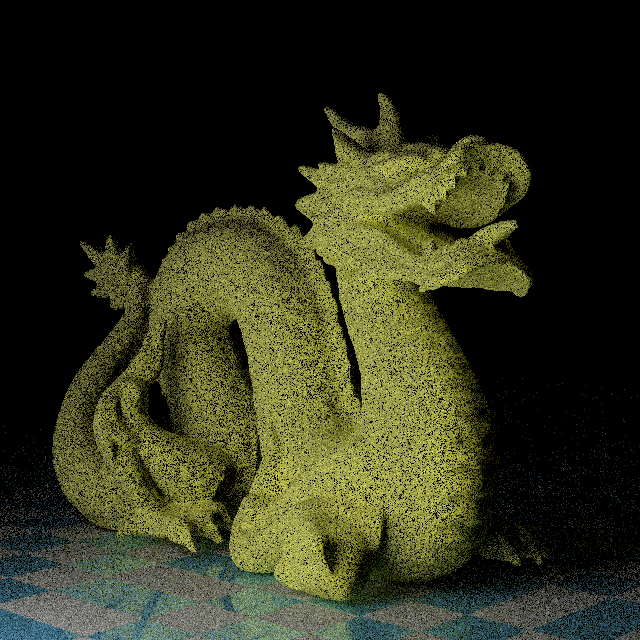
\includegraphics[width=\linewidth]{img/dragon.png}
\captionof*{figure}{dragon.scene}
\end{minipage}
\begin{minipage}{0.48\linewidth}
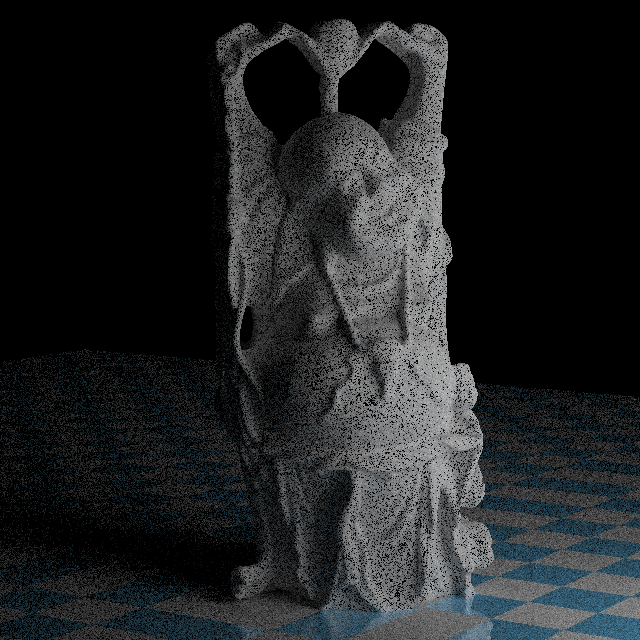
\includegraphics[width=\linewidth]{img/fatty.png}
\captionof*{figure}{buddha.scene}
\end{minipage}
\end{center}

\begin{center}
\begin{minipage}{0.48\linewidth}
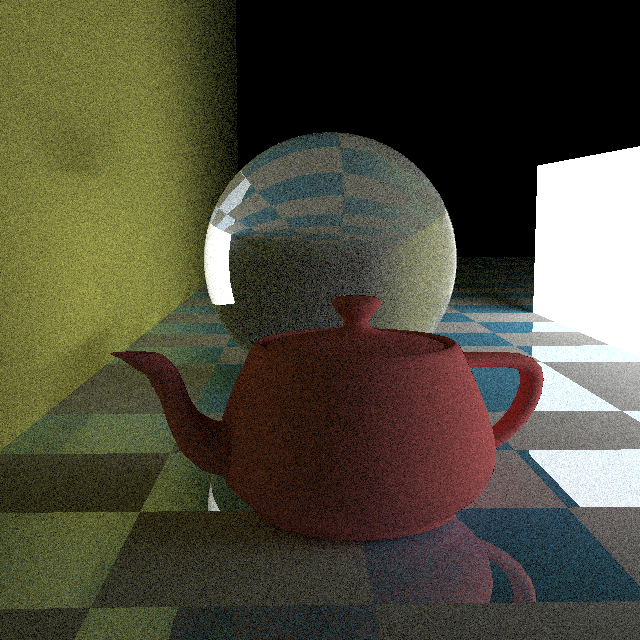
\includegraphics[width=\linewidth]{img/teapot-in-front-of-sphere.png}
\captionof*{figure}{teapot.scene}
\end{minipage}
\begin{minipage}{0.48\linewidth}
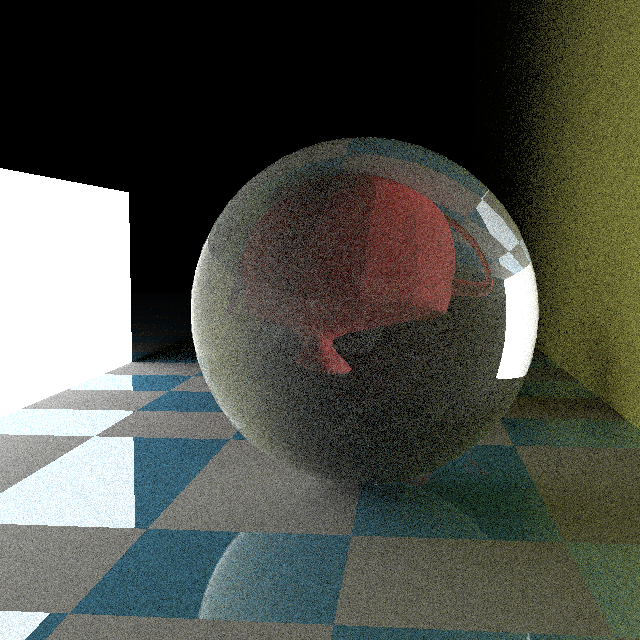
\includegraphics[width=\linewidth]{img/teapot-through-sphere.png}
\captionof*{figure}{the teapot as seen through the glass sphere}
\end{minipage}
\end{center}

\begin{center}
\begin{minipage}{0.48\linewidth}
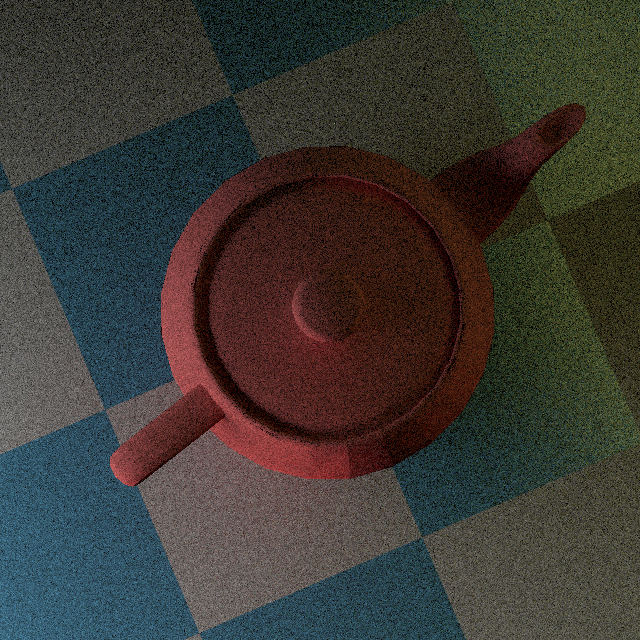
\includegraphics[width=\linewidth]{img/teapot-top.png}
\captionof*{figure}{teapot as seen from the top}
\end{minipage}
\begin{minipage}{0.48\linewidth}
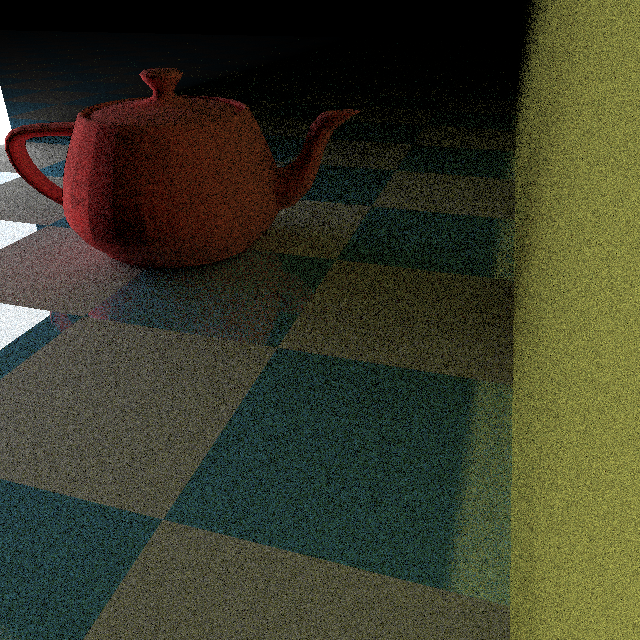
\includegraphics[width=\linewidth]{img/wall.png}
\captionof*{figure}{such indirect lighting!}
\end{minipage}
\end{center}

\begin{center}
\begin{minipage}{0.48\linewidth}
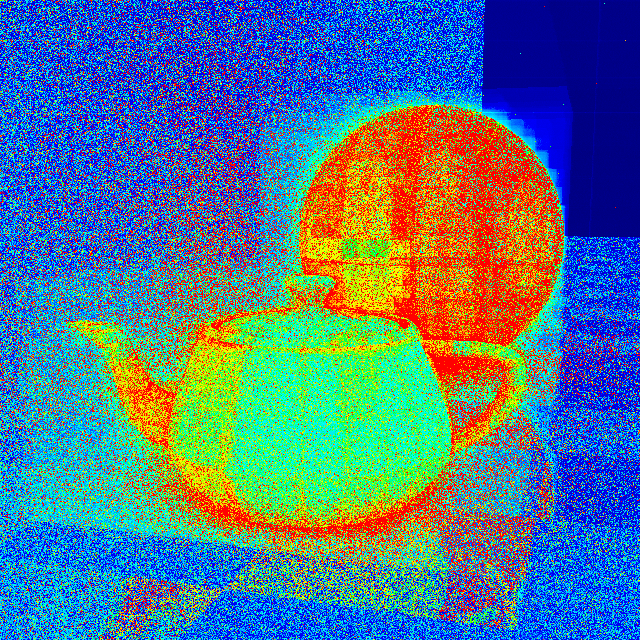
\includegraphics[width=\linewidth]{img/teapot-perf.png}
\captionof*{figure}{performance view of teapot}
\end{minipage}
\begin{minipage}{0.48\linewidth}
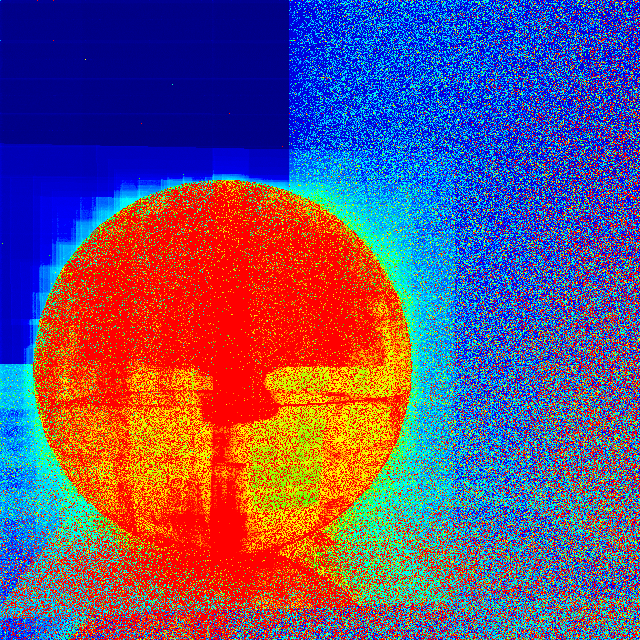
\includegraphics[width=\linewidth]{img/sphere-perf.png}
\captionof*{figure}{performance view of teapot through the sphere}
\end{minipage}
\end{center}
